% ADZE manual.
%
% Build:  make -C doc          (or: pdflatex ADZE_Manual; twice, for the TOC)
%
% The option reference in section 4.2 is generated from the OPTIONS table in
% src/ADZE_pfile.cpp by doc/gen_options.py -- do not write option
% documentation by hand here.
\documentclass[11pt]{article}

\usepackage[margin=1in]{geometry}
\usepackage{amsmath}
\usepackage{amssymb}
\usepackage{graphicx}
\usepackage{booktabs}
\usepackage{enumitem}
\usepackage{fancyvrb}
\usepackage[hidelinks]{hyperref}

% Long \texttt option names cannot hyphenate; let TeX stretch the line a
% little rather than run into the margin.
\emergencystretch=2em

\newcommand{\prog}{\textsc{adze}}
\newcommand{\structureprog}{\textsc{structure}}
\newcommand{\flag}[1]{\texttt{#1}}

\title{\prog: Allelic Diversity Analyzer\\Version 2.0}
\author{
  Zachary A. Szpiech\\
  \and
  Mattias Jakobsson\\
  \and
  Noah A. Rosenberg
}
\date{}

\begin{document}
\maketitle

\begin{abstract}
\noindent
\prog\ implements a rarefaction approach to estimating allelic richness,
private allelic richness, and private allelic richness for combinations of
populations, correcting for differences in sample size between populations.
Version 2.0 computes the same estimators as version 1.0 --- results are
identical to the last bit --- but reads its data in one pass, caches the
rarefaction probabilities, parallelizes over loci, and replaces the parameter
file with a conventional command-line interface. Section~\ref{sec:changes}
lists everything that changed.
\end{abstract}

\tableofcontents
\newpage

\section{Introduction}
\label{sec:intro}

The analysis of the distributions of alleles across populations is important
for elucidating genetic diversity and population relationships. Two
fundamental quantities for a population at a given locus are the number of
distinct alleles in the population and the number of alleles found in that
population and no other. Both are strongly dependent on sample size: a larger
sample of gene copies is more likely to contain any given allele, so counts
taken from samples of different sizes cannot be compared directly.

Rarefaction addresses this by computing, for a standardized sample size $g$,
the expected number of alleles that \emph{would} be observed if $g$ gene
copies were drawn from each population. The estimators \prog\ computes are
exact expectations under sampling without replacement, not resampling
averages, so no random number generator and no seed are involved.

\prog\ implements these computations for allelic richness, private allelic
richness, and a generalization of private allelic richness to combinations of
populations, as described in Szpiech et al. (2008).

\subsection{Allelic richness}

Consider a locus with $I$ distinct alleles, and define $N_{ij}$ as the number
of copies of allele type $i$ in a sample from population $j$. Let
$N_j = \sum_{i=1}^{I} N_{ij}$ be the sample size of population $j$ at the
locus. The probability of finding no copies of allele type $i$ in a subsample
of $g$ gene copies from population $j$ is
\begin{equation}
  Q_{ijg} = \frac{\binom{N_j - N_{ij}}{g}}{\binom{N_j}{g}}.
\end{equation}
The probability of finding at least one copy of allele type $i$ in a sample of
size $g$ from population $j$ is $P_{ijg} = 1 - Q_{ijg}$, and
\begin{equation}
  \hat{\alpha}_g^{(j)} = \sum_{i=1}^{I} P_{ijg}
\end{equation}
is the estimated allelic richness of a sample of size $g$ from population $j$
(Hurlbert, 1971; Petit et al., 1998; Kalinowski, 2004). Equation~2 estimates
the expected number of distinct alleles that will be observed in population
$j$ in a sample of size $g$.

\subsection{Private allelic richness}

Using this notation, the estimated private allelic richness for a sample of
size $g$ from population $j$ is
\begin{equation}
  \hat{\pi}_g^{(j)} = \sum_{i=1}^{I}
    \left[ P_{ijg} \left( \prod_{\substack{j'=1 \\ j' \neq j}}^{J}
      Q_{ij'g} \right) \right],
\end{equation}
where $J$ is the total number of populations (Kalinowski, 2004). This formula
sums over distinct allele types $i$ the probability that a random subsample of
size $g$ from population $j$ contains allele type $i$ and that subsamples of
size $g$ from the remaining populations do not.

\subsection{Private allelic richness for a combination of populations}

Generalizing the concept of private allelic richness, we can consider the
number of distinct alleles private to some combination of $k$ populations
selected from $\{1, 2, \ldots, J\}$. Let $S = \{1, 2, \ldots, J\}$ and let
$C_k$ be the set of all combinations of $k$ elements from $S$; there are
$\binom{J}{k}$ of them. Labelling these combinations $C_{km}$, where $m$
ranges from 1 to $\binom{J}{k}$, the estimated number of distinct alleles
private to the $m$th combination of $k$ populations, when samples of size $g$
are drawn from each of the $J$ populations, is
\begin{equation}
  \hat{\pi}_{gk}^{(m)} = \sum_{i=1}^{I}
    \left[ \left( \prod_{j \in C_{km}} P_{ijg} \right)
           \left( \prod_{j' \in S \setminus C_{km}} Q_{ij'g} \right) \right].
\end{equation}
Here $S \setminus C_{km}$ denotes the set $S$ excluding the elements of
$C_{km}$. For $k = 1$, $\hat{\pi}_{gk}^{(m)}$ reduces to private allelic
richness as in Equation~3. For $k = J-1$, Equation~4 can be considered a
measure of ``missing allelic richness'', and it reduces to
\begin{equation}
  \hat{\mu}_g^{(j)} = \sum_{i=1}^{I}
    \left[ Q_{ijg} \left( \prod_{\substack{j'=1 \\ j' \neq j}}^{J}
      P_{ij'g} \right) \right],
\end{equation}
the expected number of alleles absent from population $j$ but present in every
other population.

\subsection{Summary statistics}
\label{sec:summarystats}

\prog\ evaluates Equations~2--4 at each of many loci in a data set, and its
primary method of reporting results gives the mean, variance, and standard
error of the mean across these loci. Locus-specific estimates can also be
written out (section~\ref{sec:fulldata}). The mean across loci is calculated at
each $g$ and for each population or population grouping as
\begin{equation}
  \bar{x} = \frac{1}{L} \sum_{\ell=1}^{L} x_\ell,
\end{equation}
where $L$ is the number of loci used in the calculation and $x_\ell$ is one of
the statistics above evaluated at locus $\ell$. The variance across loci is
\begin{equation}
  s^2 = \frac{1}{L-1} \sum_{\ell=1}^{L} (x_\ell - \bar{x})^2,
\end{equation}
and the standard error of the mean is
\begin{equation}
  \mathrm{SE} = \frac{s}{\sqrt{L}}.
\end{equation}
A statistic is reported at a given $g$ only if it is defined at that $g$ for
every locus used, which requires $g \leq N_j$ at each locus for the grouping
concerned. With a single locus ($L = 1$) the variance and standard error are
undefined and are reported as \texttt{nan}.

\section{Getting started}

\subsection{Obtaining \prog}

Source is at \url{https://github.com/szpiech/ADZE}. Version 2.0 requires
nothing but a C++17 compiler. Two libraries are used when the toolchain
provides them, and the program builds and runs without either: OpenMP for
\flag{--threads}, and zlib for compressed input. Without zlib a \texttt{.gz}
file is refused with a message rather than misread.

\subsection{Building}

With CMake:
\begin{Verbatim}[xleftmargin=1em]
cmake -S . -B build -DCMAKE_BUILD_TYPE=Release
cmake --build build -j
cmake --install build --prefix ~/.local      # optional
\end{Verbatim}

\noindent Or with plain \texttt{make}:
\begin{Verbatim}[xleftmargin=1em]
make -C src                  # serial, no compressed input
make -C src OPENMP=1 ZLIB=1  # GCC, or clang on Linux
make -C src OPENMP=1 ZLIB=1 OMPFLAGS="-Xpreprocessor -fopenmp" OMPLIBS=-lomp
                             # Apple clang, with libomp installed
\end{Verbatim}

\noindent CMake reports at configure time which of the two it found; the
\texttt{make} build takes each as a flag. Without OpenMP, \flag{--threads} is
accepted but warns that it is being ignored.

\subsection{Running}
\label{sec:running}

There are two ways to specify a run, and they can be mixed:
\begin{Verbatim}[xleftmargin=1em]
adze --data mydata.stru --group-col 5 --out-prefix mypops
adze myparamfile.txt --tolerance 0.05
\end{Verbatim}

\noindent The first form takes everything from the command line. The second
reads a parameter file in the version 1.0 format --- the same keywords, and the
same short flags --- with command-line options taking precedence over the file.
Three sources are consulted, in increasing order of precedence: built-in
defaults, then the parameter file if one is given, then the command line.

\flag{--help} lists every option; \flag{--version} prints the version and the
method reference. Both work with no data file and no parameter file.
\flag{--write-template} writes a commented parameter file that runs as it
stands once \texttt{DATA\_FILE} is filled in.

Only the data file is strictly required. Everything else either has a default
or is measured from the data (section~\ref{sec:autodetect}).

\section{Input}

\subsection{Choosing a format}

Two input formats are read: the \structureprog-like layout that \prog\ has
always taken (section~\ref{sec:format}), and VCF (section~\ref{sec:vcf}),
optionally compressed with \texttt{gzip} or \texttt{bgzip}. \flag{--format}
selects one; its default, \texttt{auto}, reads the file name --- anything
ending \texttt{.vcf}, after an optional \texttt{.gz} or \texttt{.bgz}, is
treated as VCF.

The two paths converge immediately: both reduce each locus to per-grouping
allele counts and missing-data tallies, which is all the estimators use, and
both lay those counts out identically for the same genotypes. Results
therefore do not depend on which format the data arrived in --- the same
genotypes written both ways produce byte-identical output, which
\texttt{test/formats.py} checks.

\subsection{\structureprog\ format}
\label{sec:format}

This file is expected in the same format used by \structureprog: one row
per gene copy, so a diploid individual occupies two consecutive rows, preceded
by a header row of locus names. Each data row begins with one or more label
columns and continues with one allele code per locus. Allele codes are
arbitrary tokens --- integers, as in the example below, or any other strings
that do not contain whitespace.

Figure~\ref{fig:datafile} shows \texttt{example/small\_data.stru}, distributed
with \prog: five loci, three groupings, and eleven diploid individuals, with
missing alleles coded \texttt{-9}.

\begin{figure}[htbp]
\begin{Verbatim}[fontsize=\small,frame=single]
D12S1638 D14S1007 D9S1779 D9S1825 D7S2477
1037 87 Pima Mexico AMERICA 126 128 124 -9 142
1037 87 Pima Mexico AMERICA 126 128 142 -9 142
1038 87 Pima Mexico AMERICA 120 124 124 129 142
1038 87 Pima Mexico AMERICA 126 128 152 137 142
   ...
1357 24 Basque France EUROPE 126 120 124 -9 154
1357 24 Basque France EUROPE 128 122 126 -9 156
   ...
747 684 Japanese Japan EAST_ASIA 126 -9 124 129 158
747 684 Japanese Japan EAST_ASIA 128 -9 144 135 158
   ...
\end{Verbatim}
\caption{The distributed example data file, abridged. Row~1 holds the locus
names; each subsequent row is one gene copy, with five label columns followed
by five allele codes.}
\label{fig:datafile}
\end{figure}

\subsection{Dimensions are measured, not declared}
\label{sec:autodetect}

Version 1.0 required \texttt{LOCI}, \texttt{DATA\_LINES},
\texttt{NON\_DATA\_ROWS} and \texttt{NON\_DATA\_COLS} to be supplied by hand,
and validated them against the file. Version 2.0 measures them while reading:

\begin{description}[style=nextline,leftmargin=1em]
\item[\flag{--loci}] from the number of names in the header row.
\item[\flag{--data-lines}] by counting data rows.
\item[\flag{--non-data-cols}] from the width of the first data row minus the
  locus count.
\item[\flag{--group-col}] defaults to the last label column.
\item[\flag{--non-data-rows}] defaults to 1, the locus-name row. This is the
  one value that cannot be inferred, so give it explicitly if the file has
  additional header rows.
\item[\flag{--max-g}] defaults to the largest standardized sample size the
  data supports, which is the smallest $N_j$ over all groupings and all
  \emph{surviving} loci --- resolved after missing-data filtering, since
  dropping loci can raise it.
\end{description}

Any of these may still be given, in which case the declared value is used and
a warning is printed if it disagrees with what was measured. \flag{--dry-run}
reports the detected layout, the per-grouping sample sizes, the largest
feasible \texttt{MAX\_G} and the number of tuples an analysis would evaluate,
then exits without computing anything.

\subsection{VCF format}
\label{sec:vcf}

Each record is one locus and each allele index is one allele type, so the
reference allele is allele 0 and the alternates follow. A sample contributes as
many gene copies as its \texttt{GT} field holds, which lets haploid and diploid
records sit in the same file, and a \texttt{.} is an uncalled copy. A sample's
ploidy is the largest number of alleles any of its \texttt{GT} fields holds,
since that is how many gene copies it could have contributed; a record where it
carries fewer --- a haploid call in an otherwise diploid file, say --- counts
the difference as missing, and so tells against that locus under
\flag{--tolerance}. Only
\texttt{GT} is read: no other \texttt{FORMAT} field, and no \texttt{INFO},
\texttt{QUAL} or \texttt{FILTER} value, affects the counts, so filtering must
be done before \prog\ sees the file. Locus names come from the \texttt{ID}
column, or from \texttt{CHROM:POS} where \texttt{ID} is \texttt{.}.

A VCF names its samples but says nothing about which population each belongs
to, so \flag{--samples} is required with VCF input. It takes a file of two
whitespace-separated columns, sample name then grouping name:

\begin{Verbatim}[xleftmargin=1em]
# sample        grouping
HG00096         GBR
HG00097         GBR
NA18939         JPT
\end{Verbatim}

\noindent Anything after \texttt{\#} is a comment and any further columns are
ignored, so an existing sample sheet can usually be passed as it stands.
Groupings are numbered in the order they first appear in this file, which is
the order they appear in the output. A sample in the VCF that the map does not
mention is skipped, and a sample the map names that the VCF does not contain is
ignored; both are reported as warnings with a count.

Because a sample's gene copies are what the missing-data fraction is measured
against, \flag{--tolerance} means the same thing here as for
\structureprog\ input: the fraction of a grouping's gene copies that are not
called at that locus (section~\ref{sec:tolerance}).

\begin{Verbatim}[xleftmargin=1em]
adze --data cohort.vcf.gz --samples populations.tsv \
     --tolerance 0.05 --out-prefix cohort
\end{Verbatim}

\noindent \texttt{NON\_DATA\_ROWS}, \texttt{NON\_DATA\_COLS} and
\texttt{GROUP\_BY\_COL} describe the \structureprog\ layout and are ignored,
with a warning, for VCF input.

\subsection{Groupings}

With \structureprog\ input, rows are grouped by the value in the
\flag{--group-col} label column; with VCF input the grouping comes from
\flag{--samples}. In both cases groupings appear in output in the order they
are first seen;
any label column can be used, so a file annotated with population, region and
continent can be analysed at any of those levels without being rewritten, and
the same VCF can be analysed at several levels by swapping the map file.
\flag{--pops} restricts the analysis to a comma-separated list of groupings and
\flag{--exclude-pops} removes them; both change $J$, and therefore change what
``private'' means, so they are a way of asking a different question rather than
a way of subsetting output.

\subsection{Missing data and locus filtering}
\label{sec:tolerance}

An allele code equal to \flag{--missing} (default \texttt{-9}) is treated as
unobserved and reduces $N_j$ at that locus. Because a statistic is reported at
a given $g$ only when it is defined at every locus, one locus with a small
$N_j$ limits the whole analysis.

\flag{--tolerance} $x$ drops any locus at which some grouping has more than a
fraction $x$ of its gene copies missing. The default, $x = 1$, keeps every
locus. Loci dropped this way are listed in the \texttt{\_deletedloci} file
(section~\ref{sec:deletedloci}). Filtering is a trade: it discards loci to buy
a larger \texttt{MAX\_G}, and section~\ref{sec:examplesmall} works through the
trade-off on the example data.

A locus at which no allele is observed in any grouping contributes nothing;
such loci are counted, reported in a warning, and treated as undefined at
every $g$. If filtering removes every locus, \prog\ stops with an error rather
than reporting statistics over no data.

\section{Parameters and options}

\subsection{Parameter file syntax}

A parameter file is a sequence of lines, each a keyword followed by its value:
\begin{Verbatim}[xleftmargin=1em]
DATA_FILE small_data.stru
GROUP_BY_COL 5
MAX_G 8
TOLERANCE 0.24
# everything after a hash is a comment
\end{Verbatim}

\noindent Anything after \texttt{\#} is ignored. The value is the rest of the
line with surrounding whitespace removed, so values may contain spaces and may
contain other keywords as substrings. Boolean parameters take \texttt{0} or
\texttt{1}.

\subsection{Option reference}
\label{sec:options}

The following is generated from the option table in the source, so it lists
exactly what the program accepts. Each entry gives the long option, the
version 1.0 short flag where one exists, and the parameter-file keyword where
one exists.

\input{options.tex}

\section{Output}

By default \prog\ writes \texttt{adze.richness}, \texttt{adze.private} and
\texttt{adze.summary.txt} in the current directory; \flag{--out-prefix}
replaces the \texttt{adze} stem. Giving an explicit name with
\flag{--out-richness}, \flag{--out-private} or \flag{--out-tuples} uses that
name literally and appends version 1.0's suffixes (\texttt{\_summary},
\texttt{\_fulldata}, \texttt{\_deletedloci}) to it.

Results go to files; progress, warnings and errors go to standard error, so
redirecting standard output captures results alone. \flag{--quiet} silences the
diagnostics. Progress bars are drawn only when standard error is a terminal.

\subsection{Allelic richness and private allelic richness}

One row per grouping per $g$: the grouping name, the $g$ at which the
statistics were computed, the number of loci used, and then the mean, variance
and standard error across those loci (Equations~6--8). Groupings are separated
by a blank line.

\begin{Verbatim}[xleftmargin=1em,fontsize=\small]
AMERICA 2 5 1.47429 0.0886378 0.133145
AMERICA 3 5 1.76929 0.264997 0.230216

EUROPE 2 5 1.68 0.0208889 0.0646357
\end{Verbatim}

\subsection{Private allelic richness of tuples}

The same layout, with the tuple's grouping names in place of the single name.
With \flag{--tuples-k} the tuple size $k$ is appended to the file name, one
file per $k$; with \flag{--tuples} the named tuples all go to one file.

\subsection{Locus-specific output}
\label{sec:fulldata}

\flag{--full-richness}, \flag{--full-private} and \flag{--full-tuples} add a
\texttt{\_fulldata} file that carries, in addition to the summary columns, the
statistic at every locus used. The first line names the columns, including one
column per locus.

\subsection{Filtered loci}
\label{sec:deletedloci}

When \flag{--tolerance} is below 1, a \texttt{\_deletedloci} file records how
many loci were dropped, the threshold applied, and the name of each dropped
locus.

\subsection{Run summary}

A \texttt{\_summary} (or \texttt{.summary.txt}) file is written on every run.
It echoes the parameters actually used --- including values that were measured
rather than declared, and \texttt{MAX\_G} when it was resolved from the data
--- and records the elapsed time at which each phase finished.

\subsection{Tab-separated output}

\flag{--tsv} writes the result files with a header row, tab separators, and
\texttt{NA} in the value columns where a statistic is undefined at that $g$.
Without it, the legacy format is used: no header, space separators, and rows
that are undefined at a given $g$ are omitted entirely. The legacy format
remains the default so that existing scripts keep working, but \flag{--tsv} is
preferable for new work, because a consumer can distinguish ``not computable
here'' from ``not run''.

\subsection{Exit status}

\begin{tabular}{ll}
\toprule
0 & success \\
2 & usage error: unknown option, missing value, contradictory request \\
3 & I/O error: a file could not be opened, read or written \\
4 & data error: the file disagrees with itself or with the parameters \\
\bottomrule
\end{tabular}

\section{Examples}

\subsection{The distributed example data set}
\label{sec:examplesmall}

The data set in Figure~\ref{fig:datafile} has five loci and three groupings.
Running it with nothing but the data file and the grouping column,
\begin{Verbatim}[xleftmargin=1em]
adze --data small_data.stru --group-col 5 --out-prefix small
\end{Verbatim}
\noindent reports on standard error
\begin{Verbatim}[xleftmargin=1em,fontsize=\small]
Read 22 gene copies at 5 loci in 3 groupings (d:h:m:s 0:0:0:0.00)
MAX_G not given; using 3, the largest the 5 surviving loci support.
\end{Verbatim}
\noindent and writes richness results that stop at $g = 3$. Three is low for 22
gene copies, and the reason is missing data rather than sample size: the
\texttt{EUROPE} grouping has six gene copies in total, but at locus
\texttt{D9S1825} three of those six are missing, leaving $N_j = 3$.
\texttt{D9S1825} is also missing 25\% of the \texttt{AMERICA} grouping, and
\texttt{D14S1007} is missing 25\% of \texttt{EAST\_ASIA}.

Filtering those two loci buys a much larger standardized sample size:
\begin{Verbatim}[xleftmargin=1em]
adze --data small_data.stru --group-col 5 --out-prefix small24 \
     --tolerance 0.24
\end{Verbatim}
\begin{Verbatim}[xleftmargin=1em,fontsize=\small]
2 loci have at least one grouping with more than 24% missing data.
MAX_G not given; using 6, the largest the 3 surviving loci support.
\end{Verbatim}
\noindent Now the analysis runs to $g = 6$, the limit set by
\texttt{EUROPE}'s sample size alone, over the three surviving loci. Which of
the two runs to prefer is a judgement about the data: the first uses all five
loci but compares populations only at $g \leq 3$; the second compares them over
a much wider range of $g$ using three loci.

The parameter file distributed with the example, \texttt{small\_paramfile.txt},
runs the same analysis in version 1.0's style, declaring all four dimensions
along with \texttt{MAX\_G 8} and \texttt{TOLERANCE 0.2}:
\begin{Verbatim}[xleftmargin=1em]
adze small_paramfile.txt
\end{Verbatim}
\noindent Its results agree with the run above wherever the two overlap, and
the private allelic richness files are identical. The richness files are not:
declaring \texttt{MAX\_G 8} reports \texttt{AMERICA} and \texttt{EAST\_ASIA}
at $g = 7$ and $8$, which their own sample sizes reach, whereas the default
stops at the largest $g$ that \emph{every} grouping supports. Private allelic
richness stops at 6 in both, because no allele can be private at a $g$ that
some grouping cannot reach.

\subsection{A larger data set}

The next example uses the data of Rosenberg et al. (2002): 1056 individuals
from 52 populations typed at 377 microsatellite loci, available at
\url{https://rosenberglab.stanford.edu/diversity.html}. Because computing
private alleles for all combinations at the population level would be
prohibitive, the published analysis groups the individuals by region instead,
which is column~5 of that file's labels and reduces the number of groupings
from 52 to 7.

The version 1.0 parameter file for this analysis (Figure~3 of the version 1.0
manual) declared \texttt{MAX\_G 70}, \texttt{DATA\_LINES 2112},
\texttt{LOCI 377}, \texttt{NON\_DATA\_ROWS 1}, \texttt{NON\_DATA\_COLS 5},
\texttt{GROUP\_BY\_COL 5}, \texttt{K\_RANGE 2-6} and \texttt{TOLERANCE 1}. In
version 2.0 the four dimensions are measured from the file, so the same run is

\begin{Verbatim}[xleftmargin=1em]
adze --data diversitydata.stru --group-col 5 --max-g 70 \
     --stat richness,private,tuples --tuples-k 2-6 \
     --out-prefix hgdp --threads 8
\end{Verbatim}

Figures~\ref{fig:hgdprich}--\ref{fig:hgdpmiss} show the published analysis of
these data: mean allelic richness against $g$, mean private allelic richness
against $g$, and mean private allelic richness for combinations of six of the
seven regions --- that is, ``missing'' allelic richness, Equation~5. These
figures are reproduced from the version 1.0 manual and were produced with
version 1.0; version 2.0 computes the same values.

Africa carries both the highest allelic richness and, by a wide margin, the
highest private allelic richness, while the Americas and Oceania have the
highest missing allelic richness --- the alleles absent there but present
everywhere else.

\begin{figure}[htbp]
\centering
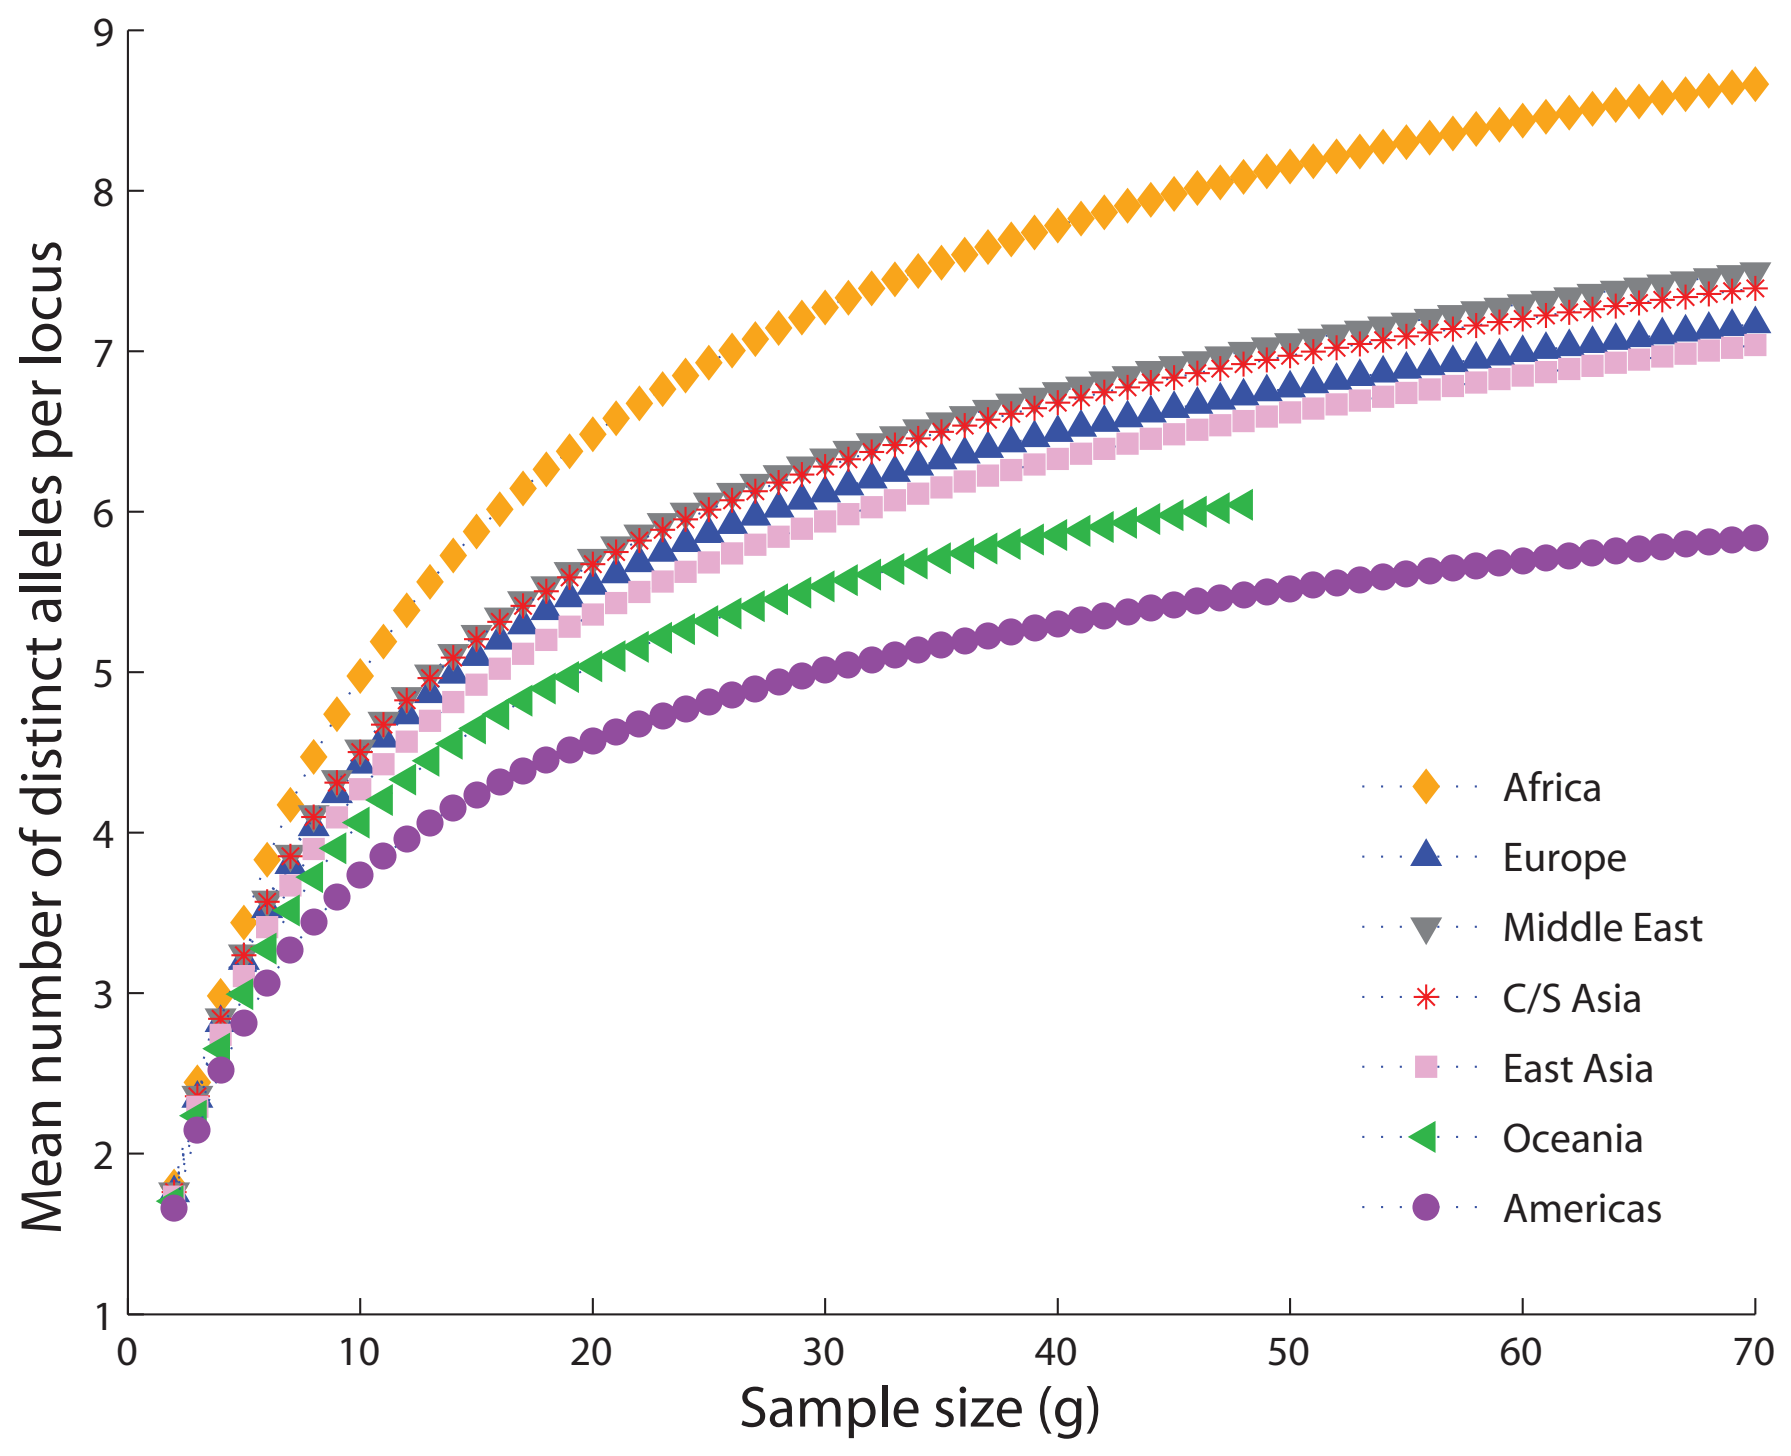
\includegraphics[width=0.82\textwidth]{figures/fig_richness_hgdp.png}
\caption{The mean number of distinct alleles per locus as a function of
standardized sample size for seven major geographic regions.}
\label{fig:hgdprich}
\end{figure}

\begin{figure}[htbp]
\centering
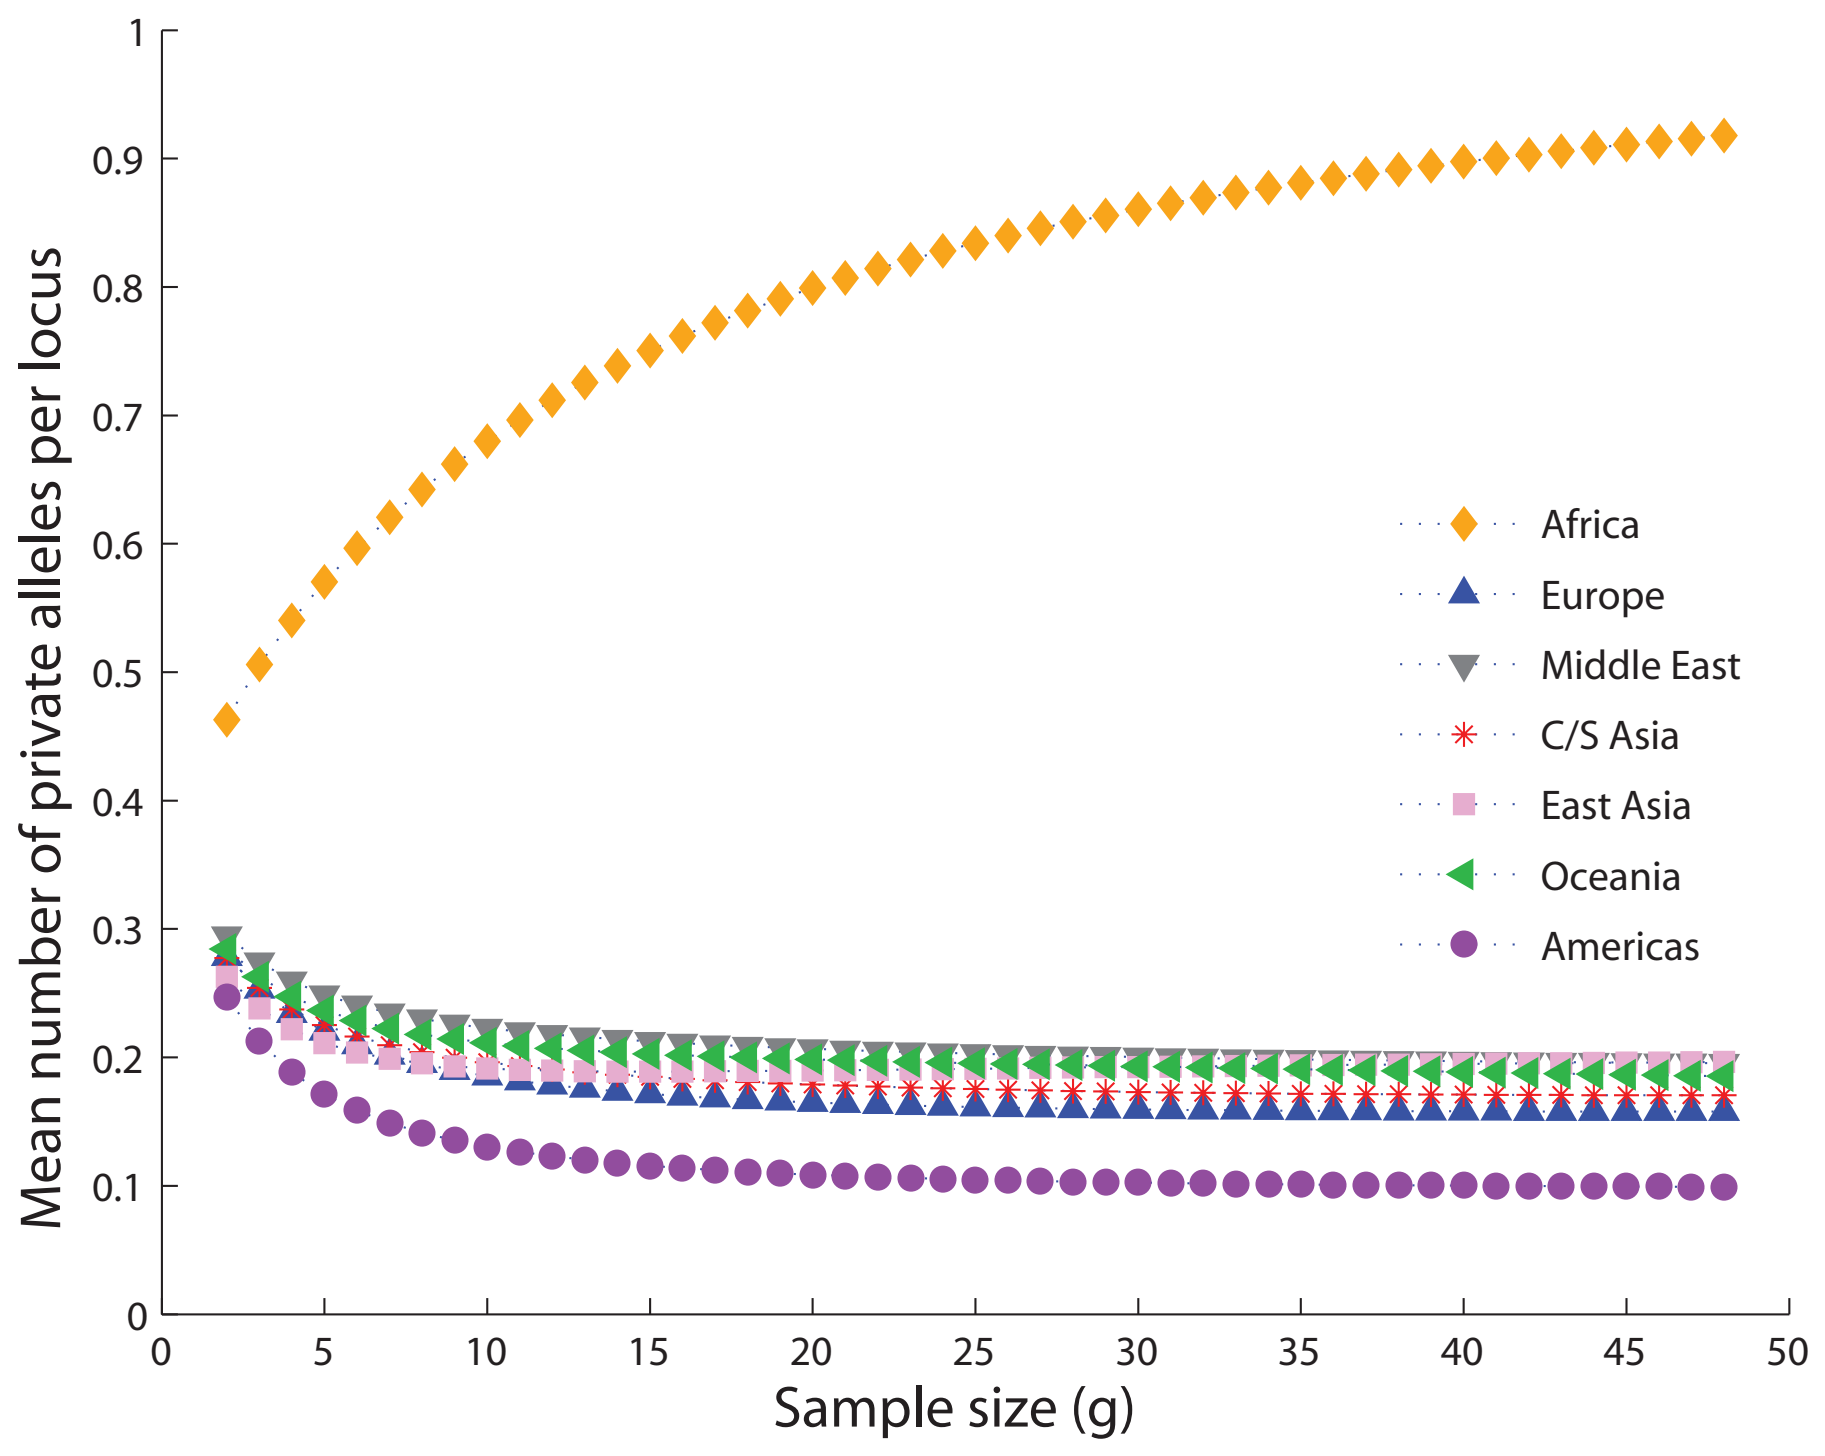
\includegraphics[width=0.82\textwidth]{figures/fig_private_hgdp.png}
\caption{The mean number of private alleles per locus as a function of
standardized sample size for seven major geographic regions.}
\label{fig:hgdppriv}
\end{figure}

\begin{figure}[htbp]
\centering
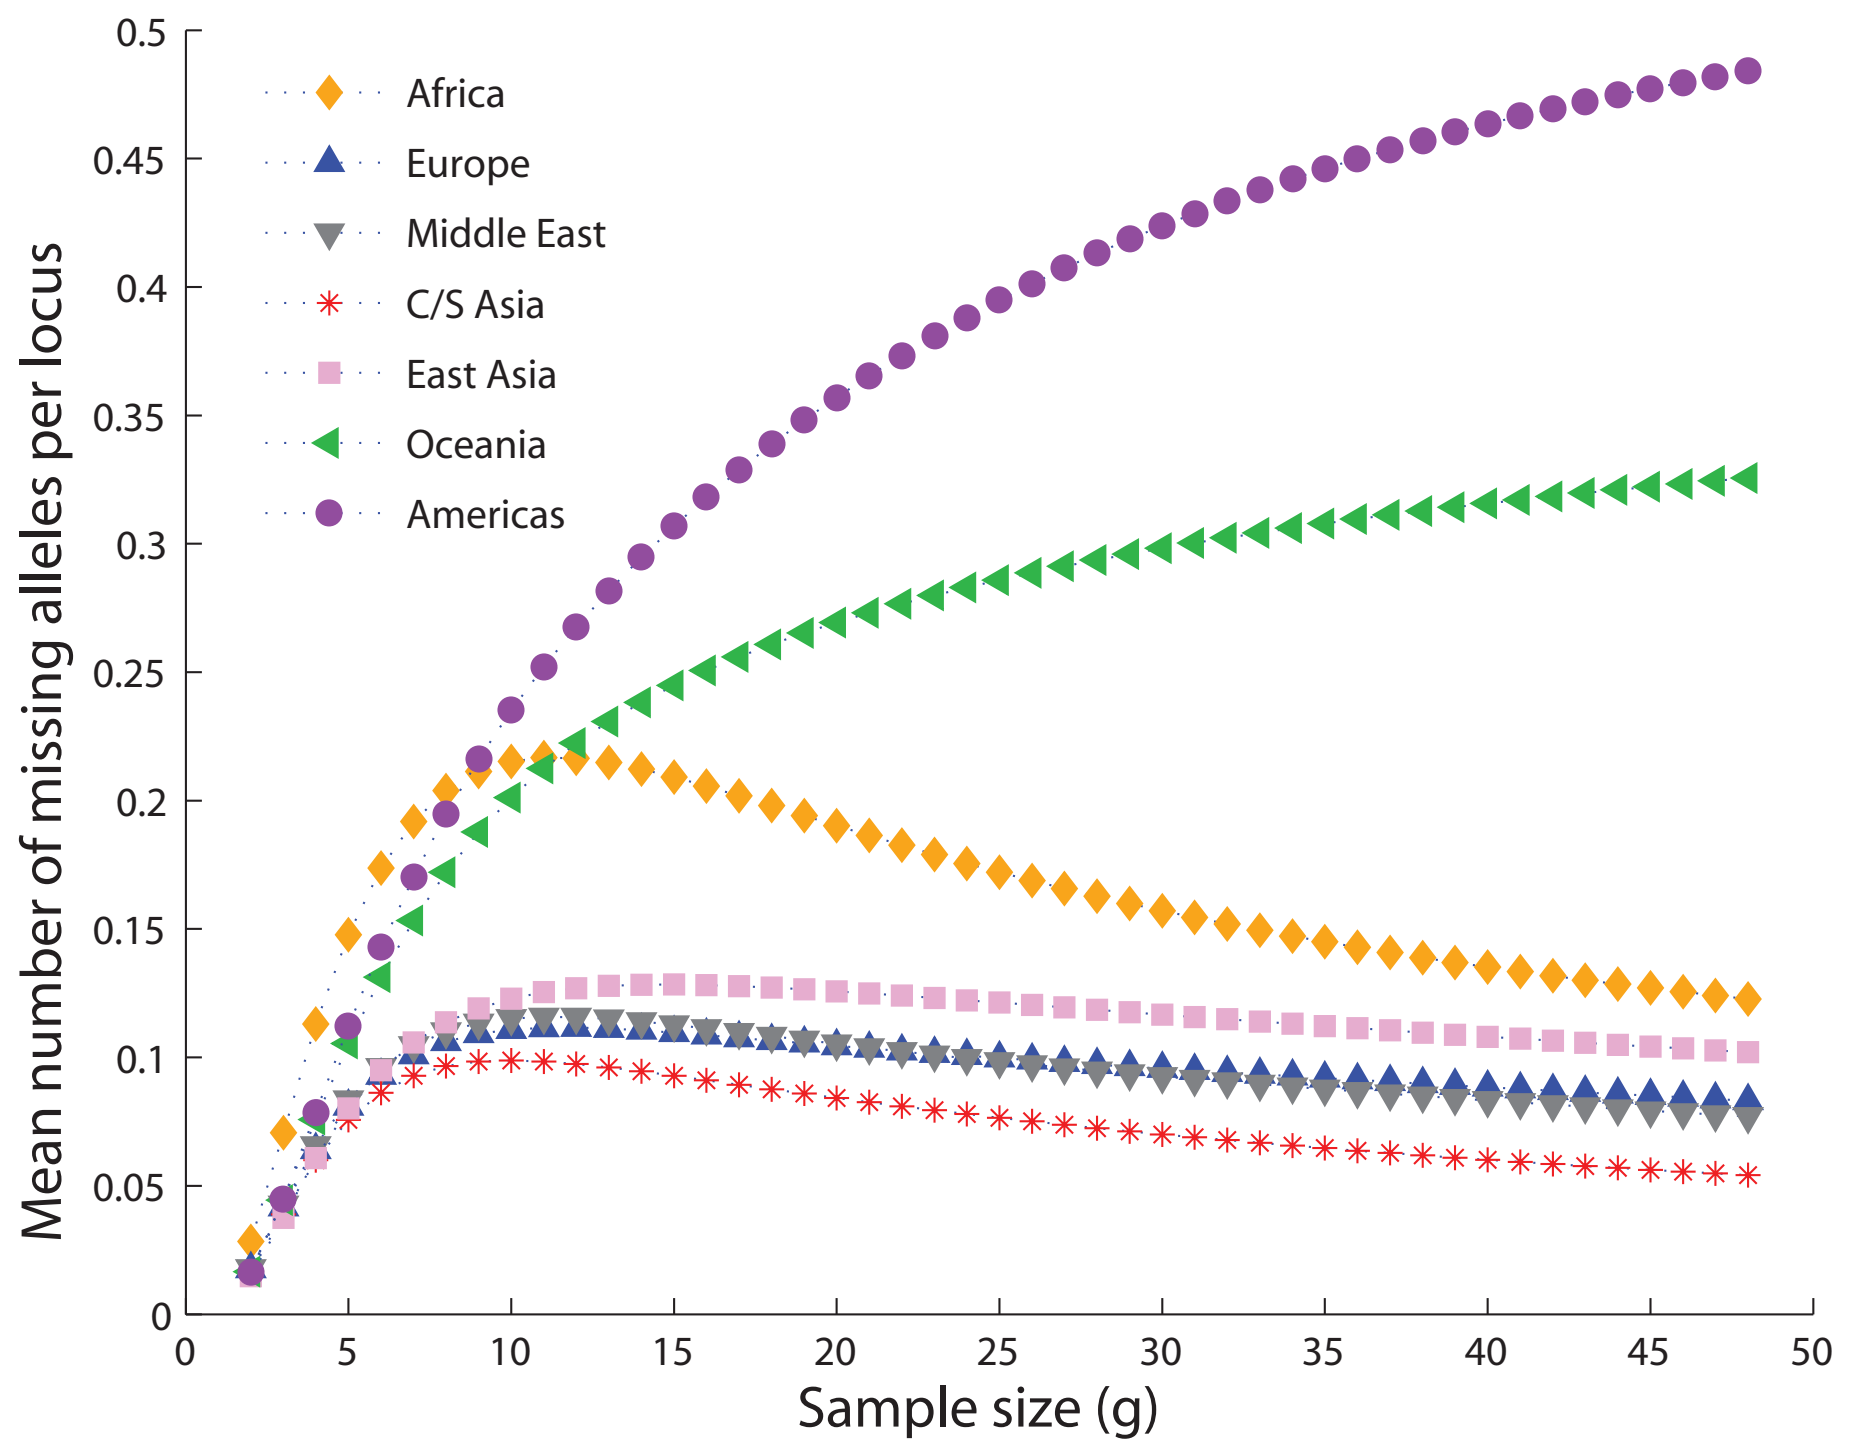
\includegraphics[width=0.82\textwidth]{figures/fig_missing_hgdp.png}
\caption{The mean number of missing alleles per locus for seven major
geographic regions (private to combinations of six of the seven regions) as a
function of standardized sample size.}
\label{fig:hgdpmiss}
\end{figure}

\subsection{Naming the tuples of interest}

A full sweep over tuple sizes evaluates $\binom{J}{k}$ combinations for each
$k$, which is $2^J$ tuples if every $k$ is requested. When only a few
groupings matter, list them in a file, one tuple per line:
\begin{Verbatim}[xleftmargin=1em]
# tuples.txt
AMERICA, EUROPE
EAST_ASIA
AMERICA, EUROPE, EAST_ASIA
\end{Verbatim}
\begin{Verbatim}[xleftmargin=1em]
adze --data small_data.stru --group-col 5 --tuples tuples.txt \
     --stat tuples --out-prefix regions
\end{Verbatim}
\noindent Each line is a comma- or space-separated list of grouping names as
they appear in the data file; \texttt{\#} starts a comment. This computes only
the tuples named, at any mixture of sizes.

\section{Performance and threading}

The per-locus loops of all three statistics can be spread over threads with
\flag{--threads} in an OpenMP build. Loci are processed independently and
reduced in locus order, so the output does not depend on the thread count: the
result files are bit-identical at any \flag{--threads} setting.

Compressed input is decompressed as it streams, so a \texttt{.vcf.gz} costs
more processor time to read than the same data uncompressed, and usually less
wall-clock time on a busy filesystem, since there is far less to transfer.

Table~\ref{tab:perf} gives the effect of the version 2.0 work on the phases
that dominate large runs, measured against a version 1.0 build on the same
inputs. The costs that grew fastest in version 1.0 were locus filtering
(quadratic in the number of loci) and the sweep over $g$ (quadratic in
\texttt{MAX\_G}); both are now linear.

\begin{table}[htbp]
\centering
\begin{tabular}{llrr}
\toprule
Phase & Condition & Version 1.0 & Version 2.0 \\
\midrule
Locus filtering & 8000 loci, 4623 dropped & 5.97 s & $<$0.01 s \\
Richness + private & 1000 loci, \texttt{MAX\_G} 80 & 4.87 s & 0.24 s \\
Tuples & 12 groupings, 495 tuples & 4.33 s & 0.67 s \\
Reading & 64 MB input & 3.62 s & 0.70 s \\
Peak memory & 64 MB input & 404 MiB & 21 MiB \\
Statistics, 8 threads & 2000 loci, \texttt{MAX\_G} 150 & --- & $4.0\times$ \\
\bottomrule
\end{tabular}
\caption{Measured on an 8-core machine, best of two runs. Version 1.0 held
every genotype in memory, so its footprint grew with sample size; version 2.0
keeps allele counts only, and its footprint is flat in the number of gene
copies.}
\label{tab:perf}
\end{table}

\section{Changes from version 1.0}
\label{sec:changes}

\subsection{Compatibility}

Parameter files written for version 1.0 work unchanged, as do the short flags.
Explicitly named output files keep version 1.0's literal suffixes, and the
default result format is unchanged. \texttt{SKIP\_CHK} and \flag{--no-check}
are still accepted but do nothing, because validation now costs nothing: it
happens during the single read pass.

\subsection{Interface}

\begin{itemize}[leftmargin=1.2em]
\item Options can be given without a parameter file, and \flag{--help} and
  \flag{--version} work with no arguments at all. A bare invocation prints
  usage; version 1.0 wrote a template parameter file into the working
  directory.
\item The parameter-file parser reads a keyword and the rest of the line.
  Version 1.0 searched each line for any keyword as a substring, so a value
  that contained a keyword --- \texttt{R\_OUT out\_LOCI\_richness} --- was
  rejected, and values could not contain spaces.
\item Dimensions are measured rather than declared
  (section~\ref{sec:autodetect}).
\item Diagnostics and progress go to standard error; exit status distinguishes
  usage, I/O and data errors.
\item VCF input, plain or \texttt{gzip}/\texttt{bgzip} compressed, via
  \flag{--format} and \flag{--samples} (section~\ref{sec:vcf}). Version 1.0
  read only the uncompressed \structureprog\ layout.
\item New: \flag{--out-prefix}, \flag{--stat}, \flag{--pops},
  \flag{--exclude-pops}, \flag{--tuples}, \flag{--tsv}, \flag{--dry-run},
  \flag{--threads}, \flag{--quiet}.
\end{itemize}

\subsection{Behaviour}

Estimates are unchanged. The following differ, in each case because version 1.0
gave an answer that could not be used:

\begin{enumerate}[leftmargin=1.5em]
\item A locus with no observed allele in any grouping is reported as undefined,
  with a warning. Version 1.0 stopped with a segmentation fault.
\item Filtering that removes every locus is an error. Version 1.0 continued and
  printed \texttt{nan} rows over zero loci.
\item A data row whose column count is wrong is always an error. With checking
  disabled, version 1.0 would misread it silently.
\item The variance of a single locus is reported as \texttt{nan} rather than
  the result of dividing by zero.
\item Reported times are elapsed wall-clock times with two decimals. Version
  1.0 reported processor time truncated to whole seconds, which is why the
  example run in the version 1.0 manual reports \texttt{0:0:0:0} throughout.
\end{enumerate}

\subsection{Verification}

Every change was checked with a differential test that runs version 2.0 and a
version 1.0 build over the same inputs and compares every output file byte for
byte: nine synthetic data sets --- spanning allele-count range, missingness, a
single locus, a single grouping, unequal sample sizes, haploid data, and a
locus with no observed alleles --- crossed with nine parameter settings, plus
the distributed example. All 69 comparable cases are byte-identical; the
remaining cases are those in which version 1.0 crashes or reports statistics
over zero loci, and so has no output to compare. The test is in
\texttt{test/regress.py} and needs a version 1.0 binary to compare against.

VCF input has no version 1.0 counterpart, so it is checked differently:
\texttt{test/formats.py} writes one set of genotypes as \structureprog, as
VCF, and as compressed VCF, and requires the three runs to agree
byte-for-byte. Because both readers order allele slots by the same rule, the
comparison is exact rather than approximate --- any difference at all is a
real one, not a change in the order of a floating-point sum.

\section*{References}
\addcontentsline{toc}{section}{References}

\begin{itemize}[label={},leftmargin=1.5em,itemindent=-1.5em]
\item Hurlbert, S. H. 1971. The nonconcept of species diversity: a critique and
  alternative parameters. \textit{Ecology} 52: 577--586.
\item Kalinowski, S. T. 2004. Counting alleles with rarefaction: private alleles
  and hierarchical sampling designs. \textit{Conservation Genetics} 5: 539--543.
\item Kalinowski, S. T. 2005. \textsc{hp-rare} 1.0: a computer program for
  performing rarefaction on measures of allelic richness.
  \textit{Molecular Ecology Notes} 5: 187--189.
\item Petit, R. J., A. El Mousadik, and O. Pons. 1998. Identifying populations
  for conservation on the basis of genetic markers.
  \textit{Conservation Biology} 12: 844--855.
\item Rosenberg, N. A., J. K. Pritchard, J. L. Weber, H. M. Cann, K. K. Kidd,
  L. A. Zhivotovsky, and M. W. Feldman. 2002. Genetic structure of human
  populations. \textit{Science} 298: 2381--2385.
\item Szpiech, Z. A., M. Jakobsson, and N. A. Rosenberg. 2008. \prog: a
  rarefaction approach for counting alleles private to combinations of
  populations. \textit{Bioinformatics} 24: 2498--2504.
\end{itemize}

\end{document}
